\chapter{Ознакомительная}
\textbf{Цель:} Запустить плату, подключиться к ней через консоль и по сетевому интерфейсу, работа с кнопкой и светодиодами через sysfs.

\vspace{5mm}
\textbf{Описание:} работа с ОС Linux на целевой платформе мало чем отличается от работы с данной ОС на обычном компьютере. Среди особенностей можно выделить наличие меньшего набора инструментов, и рабочих программ, что делается для экономии свободного места, и ускорения загрузки ОС. Так же может отсутствовать привычный рабочий стол, а вся работа сводиться к взаимодействию через рабочий терминал, она же консоль. Для подключения к консоли можно воспользоватся интерфейсом UART (он же COM порт, или последовательный порт), или при помощи сетевого соединения (ssh или реже telnet). 

При этом нужно понимать, что возможность работы через консоль настраивается, и не всегда может быть доступна по-умолчанию (обычно возможность сетевого подключения отключают, для повышения безопасности). 

\vspace{5mm}
\textbf{Полезные ссылки:}
\begin{enumerate}
	\item \href{https://habr.com/ru/sandbox/166705/}{Хабр: Коротко об SSH}.
	\item \href{https://man7.org/linux/man-pages/man5/sysfs.5.html}{man7.org: sysfs}.
	\item \href{https://embetronicx.com/tutorials/linux/device-drivers/sysfs-in-linux-kernel/}{EmbeTronicX: sysfs}.
	\item \href{https://www.kernel.org/doc/Documentation/gpio/sysfs.txt}{Kernel Doc: GPIO Sysfs Interface for Userspace}.	
\end{enumerate}

\section{Запуск и подключение к устройству}

\subsection{}Запустите виртуальную машину. Логин и пароль для входа: student / usrstudent.

\subsection{}Подключите по USB плату к ПК. Проверьте, и при необходимости подключите USB устройство FTDI RBM\_C1K5500VK018 к виртуальной машине (меню Device→USB).

\subsection{}Откройте программу gtkterm, и подключитесь к порту /dev/ttyUSB1, или откройте консоль в виртуальной машине, и вызовете утилиту minicom.

\subsection{}Если в окне терминала нет текста, нажмите клавишу Enter на клавиатуре. В окне должен появится следующий вывод:
\begin{center}
	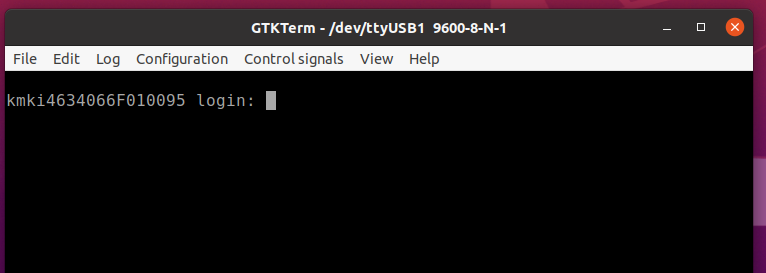
\includegraphics[width=\textwidth]{pic_08}
\end{center}
Введите логин root и пароль root.

\section{Подключение по сетевому интерфейсу}

Рассмотрим какие шаги необходимо выполнить, для того, что бы можно было организовать сетевое подключение к плате, для получение доступа к консоли и файловой системе через SSH соединение. Так же настройки, которые будут выполнены в данном разделе помогут в дальнейшем копировать файлы на плату через команду scp.

\subsection{}Проверьте текущие настройки интерфейса eth0 выполнив команду: 
\begin{lstlisting}[style=bash]
$ ip -4 addr show dev eth0 
\end{lstlisting}
Проверьте результат, IP адрес платы должен быть 192.168.100.200
\begin{lstlisting}[style=stdout]
	...
inet 192.168.100.200/24 brd ... scope global eth0 
	...
\end{lstlisting}
Результат отображает информацию по выбранному интерфейсу, в данном случае интерес представляет адрес указанный после слова inet. Это IP адрес, который присвоен плате.
 
Если inet адрес отличается, то удалите текущий адрес (вместо <inet\_val> впишите адрес, который отобразился в консоли)
\begin{lstlisting}[style=bash]
$ ip addr del <inet_val> dev eth0
\end{lstlisting}
затем установите новый адрес командой 
\begin{lstlisting}[style=bash]
$ ip addr add 192.168.100.200/24 dev eth0
\end{lstlisting} 
Для активации изменения необходимо переподключится, для чего выполните следующие команды
\begin{lstlisting}[style=bash]
$ ip link set eth0 down
$ ip link set eth0 up
\end{lstlisting} 

\subsection{}Проверьте, что на плате запущен SSH сервер. Проверить открытые порты устройства, выполнив команду: 

\begin{lstlisting}[style=bash]
$ netstat -tulpn | grep LISTEN
\end{lstlisting} 
\begin{center}
	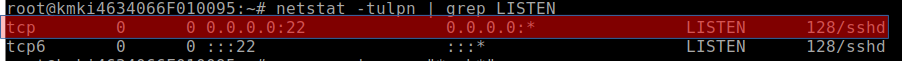
\includegraphics[width=\textwidth]{pic_09}
\end{center}
Если вывода, как на картинках выше не появилось, то выполните команду: 
\begin{lstlisting}[style=bash]
$ systemctl start sshd 
\end{lstlisting}
и проверьте снова. 

\subsection{}\label{lab2:ref1}Заходить через сеть в пользователя root не безопасно, поэтому создадим пользователя для дальнейшей работы через сетевой интерфейс, для этого введите следующие команды (пароль для пользователя netuser - usrnetuser):
\begin{lstlisting}[style=bash]
$ useradd -s /bin/bash -m netuser
$ passwd netuser
\end{lstlisting}

Первая команда для создания нового пользователя netuser с созданием домашнего каталога (/home/netuser) и также назначаем для него интерпретатора команд bash. 

\subsection{}Подключите сетевой шнур к рабочему ПК и плате

\subsection{}Откройте на виртуальной машине консоль, нажав на клавиатуре комбинацию клавиш Ctrl+Alt+T. 

\subsection{}\label{lab2:ref2}В открывшемся окне терминала введите команду: 
\begin{lstlisting}[style=bash]
# ssh netuser@192.168.100.200
\end{lstlisting}

\subsection{}Будет предложено ввести пароль пользователя, вводим тот, что установили в пункте \ref{lab2:ref1} и получаем доступ к терминалу платы.

Если вместо ввода пароля, в консоли появилась надпись похожую на:
\begin{lstlisting}[style=stdout]
The authenticity of host '192.168.100.200 (192.168.100.200)' can't be established.
ECDSA key fingerprint is SHA256:+OSEJhr2dIiTvlWZxq5fZ0UFdYYY+egbTgabe6F7zZE.
Are you sure you want to continue connecting (yes/no/[fingerprint])?
\end{lstlisting}
Введите yes и нажмите Enter, и повторно ведите пароль.
\\\\
Если же получите вывод как на картинке ниже
\begin{center}
	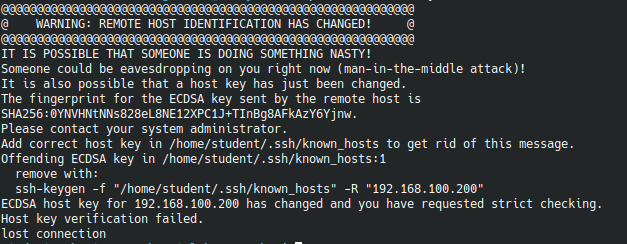
\includegraphics[width=\textwidth]{pic_10}
\end{center}
Выполните команду 
\begin{lstlisting}[style=bash]
$ ssh-keygen -f "/home/student/.ssh/known_hosts" -R "192.168.100.200"
\end{lstlisting}
и вернитесь к пункту \ref{lab2:ref2}

\subsection{}Завершите сеанс, введя команду exit 

\section{Настройка доступа по ключу}

SSH подключение можно организовать без необходимости ввода пароля, для этого используются ключи шифрования. При этом создаётся два ключа, один ключ приватный, который остаётся на машине, с которой планируется осуществлять доступ, и второй - публичный, для добавления на сервера (или удалённые системы) к которым необходимо подключится.
\begin{center}
	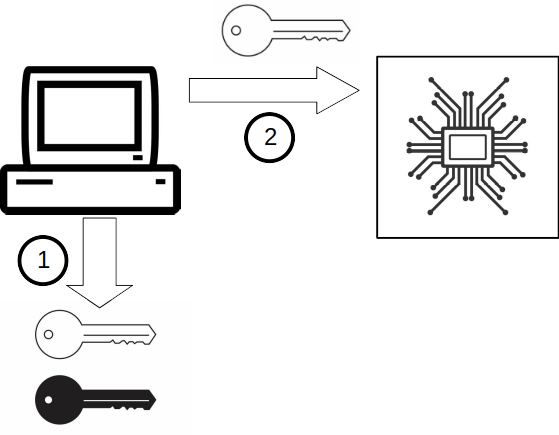
\includegraphics[width=0.4\textwidth]{ssh_desc}
\end{center}

\subsection{}В терминале виртуальной машины создаём пару из приватного и публичного ключей:
\begin{lstlisting}[style=bash]
# ssh-keygen
\end{lstlisting}

Будет задан вопрос о пути и имени файла с приватным ключом (публичный будет лежать там же, с тем же именем и дополнительным суффиксом .pub), тут оставляем поля ввода пустым, и жмём кнопку Enter.

Далее будет предложенно указать passphrase. Впишите слово \textbf{s3cr3t}\label{ssh:passphrase}, и нажмите Enter. После чего нужно будет вновь повторить его. Это по сути пароль который нужно будет указать, что бы воспользоватся созданным ключом, что позволит дополнительно обезопасить файл-ключ, так как в случае его утечки, злоумышлинику придётся дополнительно узнать эту фразу, перед тем как воспользоватся файл-ключом.  

\begin{Notes}{Запомните:}
	В данном случае, используются стандартные настройки, однако на них можно повлиять, в частности генерируемый ключ на базе RSA шифрования, с длинной ключа в 2048 бит, что считается безопасным, но до 2030 года. В случае, если плата имеет доступ в глобальную сеть, рекомендуется устанавливать длинну ключа не менее 3072 бита:
	\begin{lstlisting}[style=bash]
	# ssh-keygen -t rsa -b 3072
	\end{lstlisting}
	
	Через ключ t можно выбрать алгоритм шифрования. Информацию о доступных алгоритмах шифрования списке ключей для запуска приложения и т.д. можно получить выполнив следующую команду:
	\begin{lstlisting}[style=bash]
	# ssh-keygen --help
	\end{lstlisting}
	или
	\begin{lstlisting}[style=bash]
	# man ssh-keygen
	\end{lstlisting}
\end{Notes}


\subsection{}Копируем публичный ключ на плату
\begin{lstlisting}[style=bash]
# scp ./.ssh/id_rsa.pub netuser@192.168.100.200:/home/netuser/
\end{lstlisting}

\subsection{}Переходим в терминал платы, и допишем ключ, в файл с ключами авторизаци
\begin{lstlisting}[style=bash]
$ cat /home/netuser/id_rsa.pub >> /home/netuser/.ssh/authorized_keys
\end{lstlisting}

\subsection{}Удалим файл с публичным ключом
\begin{lstlisting}[style=bash]
$ rm /home/netuser/id_rsa.pub
\end{lstlisting}

\subsection{}Проверим попытвшись подключится к плате по ssh
\begin{lstlisting}[style=bash]
# ssh netuser@192.168.100.200
\end{lstlisting}
Если теперь запрашивает секретную фразу (passphrase) с указанием пути к приватному ключу: '/home/student/.ssh/id\_rsa' значит всё сделанно правильно.

\subsection{}Осталось завершить конфигурацию, добавив в кэш сессии виртуальной машины секретную фразу, что бы не вводить её при каждом обращении к плате:
\begin{lstlisting}[style=bash]
# ssh-add
\end{lstlisting}
впишите секретную фразу из пункта \ref{ssh:passphrase}. Теперь для входа по ssh в терминал платы, или копирования данных по ssh программой scp, не нужно будет указывать паролей или секретных фраз.  

\begin{Notes}{Запомните:}
ssh-agent это менеджер ключей для SSH. 

ssh-add позволяет добавить в "память" ssh-agent ключи. Однако эта система работает до перезагрузки виртуальной машины. При новом входе, перед первым взаимодействием с платой нужно будет добавлять ключи в "память" ssh-agent'а.
\end{Notes}

\subsection{}Финальная проверка
\begin{lstlisting}[style=bash]
# ssh netuser@192.168.100.200
\end{lstlisting}
После запроса на подключение сразу должен произойти переход в терминал платы, без запроса пароля или секртеной фразы.

\subsection{}Закрыть подключение
Завершите сессию по SSH закрыв терминал, или набрав команду. 
\begin{lstlisting}[style=bash]
$ exit
\end{lstlisting}


\section{Аппаратный Hello world }

В этой части будет показано, как можно управлять выводами микроконтроллера, для переключения светодиодов и считывания состояния кнопки, при помощи виртуальной файловой системы sysfs.

Для работы с периферией в ОС Linux помимо прочего есть две виртуальные файловые системы: procfs (точка входа /proc) и sysfs (точка входа /sys).  

Sysfs экспортирует в пространство пользователя информацию ядра Linux о присутствующих в системе устройствах и драйверах, что позволяет не только считывать значение (например с датчиков температуры), но и менять поведение, если это было заложено разработчиками драйвера.

За формирование наполнения виртуальных файловых систем отвечают в том числе и модули ядра Linux, которые выполняют роль драйвера, если речь идёт про взаимодействие с периферийным модулями.

\subsection{}Перейдите в каталог /sys/class/gpio:
\begin{lstlisting}[style=bash]
$ cd /sys/class/gpio
\end{lstlisting}

\subsection{}Выведите список фалов и каталогов в текущей директории: 
\begin{lstlisting}[style=bash]
$ ls -l
\end{lstlisting}
\begin{center}
	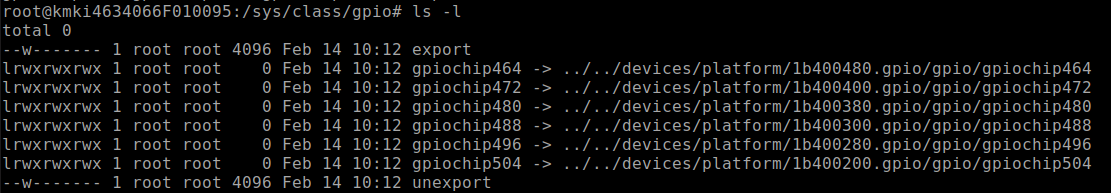
\includegraphics[width=\textwidth]{pic_11}
\end{center}

Первый и последний файлы используются для того, что бы подключать (export) драйвер для управления отдельным выводом в файловую систему sysfs или отключать (unexport). 

Далее идёт серия символьных ссылок на каталоги, каждый из которых описывает один банк сигналов ввода-вывода общего назначения (GPIO). Тут нужно отметить, что в рабочем чипе присутствует 6 банков (A, B, C, D, E и F), по 8 выводов в каждом, по этой причине мы видим 6 каталогов.  

Обратите внимание на имена каталогов, внутри каталога platform. Первая часть имени является базовым адресом периферийного модуля, отвечающего за управление банком выводов. Первому банку выводов A соответствует адрес 0x1B400200, остальные по возрастанию. 

Так же обратите своё внимание, что в данной сборке, номера файлов gpiochip уменьшаются(!), при продвижении от выводов в банке A к выводам в банке F.

\subsection{}У выводов общего назначения в рамках ядра Linux нумерация сквозная. Таким образом, можно определить, что вывод подключённый к кнопке SW2 (банк D, вывод 6) находиться под номерам 486 (480 + 6).  Выполним следующую команду:
\begin{lstlisting}[style=bash]
$ echo 486 > export
\end{lstlisting}

\subsection{}Выполните эту же команду для экспорта пары выводов банка F (464 и 465) 

\subsection{}После каждой команды будет создан каталог ./gpioXXX где вместо XXX будет номер вывода. Если зайти в любой из этих каталогов, то можно увидеть там одинаковый набор файлов, но нас интересуют следующие: 
\begin{itemize}
\item direction — задаёт направление вывода (in вывод настроен как вход, out — как выход)
\item value — если вывод настроен как вход, то читая этот файл можем узнать уровень логического сигнала на выводе. Если настроен на выход, то запись в этот файл 0 или 1 будет устанавливать соответствующий уровень выходного сигнала.
\end{itemize}

\subsection{}Так как два вывода банка F управляют светодиодами, изменим значение в файле direction  для них на out
\begin{lstlisting}[style=bash]
$ echo out > gpio464/direction
$ echo out > gpio465/direction
\end{lstlisting}

\subsection{}Переключать светодиоды можно записью 0 или 1 в файл value соответствующего вывода
\begin{lstlisting}[style=bash]
$ echo 1 > gpio464/value
$ echo 0 > gpio464/value
\end{lstlisting}

\subsection{}Для взаимодействия с кнопкой менять ничего не нужно. Для удобства отладки запустить считывание файла через утилиту watch позволяющую выполнять заданную команду через указанный интервал времени.

\begin{lstlisting}[style=bash]
$ watch -n 1 cat gpio486/value
\end{lstlisting}

После чего можете нажимать кнопку, и смотреть как меняется значение считанное из файла. В данном примере файл будет считываться каждую секунду (из-за параметра -n 1 переданного при запуске утилите watch).  

\subsection{}Остановите работу программы watch комбинацией клавиш \\ Ctrl + C

\subsection{} Выключите плату, для чего в начале введите команду
\begin{lstlisting}[style=bash]
	$ poweroff
\end{lstlisting}
дождитесь, как появиться надпись
\begin{lstlisting}[style=stdout]
	reboot: System halt
\end{lstlisting}
после чего отключите USB кабель от ПК или платы. 

\section{Задание для самостоятельной работы}
Экспортируйте все выводы банков F и E, и включите все светодиоды.

\subsubsection{*} Написать bash скрипт, который будет делать экспорт нужных выводов, если необходимо, и в зависимости от того, нажата кнопка или нет поочерёдно включать или выключать все светодиоды с задержкой в 1с между переключениями. 
